\chapter{Экспериментальная часть}

В данном разделе описаны проведённые замеры и представлены результаты исследования. Также будут уточнены характеристики устройства, на котором проводились замеры.

\section{Технические характеристики}
Технические характеристики устройства, на котором выполнялось тестирование \cite{web_item5}:
\begin{itemize}
	\item операционная система $macOS$ $Monterey$ 12.4;
	\item 8 ГБ оперативной памяти;
	\item процессор $Apple$ $M2$ (базовая частота~---~2400 МГц, но поддержка технологии $Turbo$ $Boost$ позволяет достигать частоты в 3500 МГц \cite{web_item10}).
\end{itemize}

\section{Измерение времени выполнения реализаций алгоритмов}
Замеры времени работы реализаций алгоритмов производились при помощи встроенных в Go средств, а именно «бенчмарков» ($benchmarks$ из пакета $testing$ стандартной библиотеки $Go$ \cite{web_item2}), представляющих собой тесты производительности \cite{web_item18}. Для построения графика использовалась графическая утилита $gnuplot$ \cite{web_item17}.

Значение $N$ динамически изменяется для достижения стабильного результата при различных условиях, но гарантируется, что каждый «бенчмарк» будет выполняться хотя бы одну секунду. Для замеров отправлялось количество заявок от 1 до 10, где в качестве исходных данных были тексты, написанные вручную, взятые из книг или со случайных страниц Википедии. Размеры файлов для замеров~---~до 100000 слов. Результаты тестирования возвращаются в структуре специального вида. Пример такой структуры представлен в листинге \ref{code:go_bench_struct}.

\begin{code}
\caption{Листинг структуры результата «бенчмарка»}
\label{code:go_bench_struct}

\begin{minted}{go}
testing.BenchmarkResult{N:120000, T:1200000000, Bytes:0, MemAllocs:0x0, 
MemBytes:0x0, Extra:map[string]float64{}}
\end{minted}
\end{code}

В листинге \ref{code:go_bench} представлен пример реализации «бенчмарка».
\begin{code}
\caption{Листинг примера реализации «бенчмарка»}
\label{code:go_bench}

\begin{minted}{go}
func NewBenchmarkParallel(docs []document.Document, 
rules []rule.Rule) func(*testing.B) {
	return func(b *testing.B) {
		for j := 0; j < b.N; j++ {
			pipeline.LaunchParallel(docs, rules, 0)
		}
	}
}
\end{minted}
\end{code}

В таблице \ref{table:total_time} представлены результаты замеров времени работы конвейера (в мкс.) при разном количестве входных заявок. На рисунке \ref{img:graph1} приведен график, отражающий зависимость времени выполнения реализаций конвейерных вычислений от количества заявок в очереди. В легендах графиков обозначение $Lin$ значит последовательный конвейер, а $Par$~---~параллельный.

\begin{table}[H]
  \caption{\label{table:total_time} Результаты замеров времени работы конвейера при разном количестве входных заявок (мкс.)}
  \begin{center}
    \begin{tabular}{
    |S[table-format=4.0]
    |S[table-format=10.0]
    |S[table-format=10.0]|
    }
      \hline
      {Кол-во заявок} & {Линейный конвейер} & {Параллельный конвейер} \\ \hline
      1 & 101081 & 101914\\ \hline
      2 & 197148 & 176099\\ \hline
      3 & 292401 & 246154\\ \hline
      4 & 384686 & 319440\\ \hline
      5 & 481481 & 387951\\ \hline
      6 & 575756 & 460617\\ \hline
      7 & 665199 & 528644\\ \hline
      8 & 767686 & 608424\\ \hline
      9 & 847215 & 668477\\ \hline
      10 & 940343 & 741789\\ \hline
    \end{tabular}
  \end{center}
\end{table}

\newpage

\noindent
\begin{table}[h!]
  \centering
  \begin{tabular}{p{1\linewidth}}
    \centering
    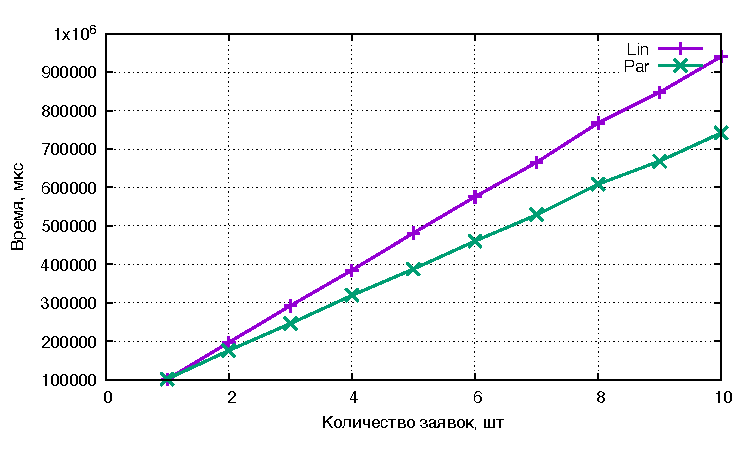
\includegraphics[width=0.6\linewidth]{./images/time.pdf}
    \captionof{figure}{Зависимость времени работы конвейера от количества входных заявок}
    \label{img:graph1}
  \end{tabular}
\end{table}

Замеры для журналирования проводились при помощи стандартной библиотеки Go \cite{web_item12}\cite{web_item15}. В таблице \ref{table:line_lin_time} представлен пример журналирования времени обработки заявок для последовательного конвейера, в таблице \ref{table:line_par_time} представлен пример журналирования времени обработки заявок для параллельного конвейера, при количестве заявок равном четырём.

\begin{table}[H]
  \caption{\label{table:line_lin_time} Пример журналирования времени работы последовательного конвейера (мкс.)}
  \begin{center}
    \begin{tabular}{
    |S[table-format=4.0]
    |S[table-format=10.0]
    |S[table-format=10.0]
    |S[table-format=10.0]|
    }
      \hline
      {№ заявки} & {Этап} & {Начало} & {Конец} \\ \hline
      1 & 1 & 46 & 71027\\ \hline
      1 & 2 & 71028 & 77461\\ \hline
      1 & 3 & 77462 & 85849\\ \hline
      2 & 1 & 85852 & 129239\\ \hline
      2 & 2 & 129240 & 134997\\ \hline
      2 & 3 & 134997 & 142526\\ \hline
      3 & 1 & 142528 & 185578\\ \hline
      3 & 2 & 185580 & 190813\\ \hline
      3 & 3 & 190813 & 198346\\ \hline
      4 & 1 & 198348 & 241285\\ \hline
      4 & 2 & 241286 & 247956\\ \hline
      4 & 3 & 247957 & 255470\\ \hline
    \end{tabular}
  \end{center}
\end{table}

\begin{table}[H]
  \caption{\label{table:line_par_time} Пример журналирования времени работы параллельного конвейера (мкс.)}
  \begin{center}
    \begin{tabular}{
    |S[table-format=4.0]
    |S[table-format=10.0]
    |S[table-format=10.0]
    |S[table-format=10.0]|
    }
      \hline
      {№ заявки} & {Этап} & {Начало} & {Конец} \\ \hline
      1 & 1 & 2 & 75155\\ \hline
      1 & 2 & 75176 & 85541\\ \hline
      1 & 3 & 85544 & 99337\\ \hline
      2 & 1 & 75159 & 149655\\ \hline
      2 & 2 & 149677 & 159719\\ \hline
      2 & 3 & 159723 & 173595\\ \hline
      3 & 1 & 149658 & 225378\\ \hline
      3 & 2 & 225398 & 235442\\ \hline
      3 & 3 & 235446 & 249523\\ \hline
      4 & 1 & 225381 & 300991\\ \hline
      4 & 2 & 300996 & 314670\\ \hline
      4 & 3 & 314674 & 328010\\ \hline
    \end{tabular}
  \end{center}
\end{table}

В таблице \ref{table:time_analyth} представлен анализ характеристик работы реализаций алгоритмов конвейеров для количества заявок, равного четырём.

\begin{table}[H]
		\renewcommand{\arraystretch}{1.4}
		\caption{\label{table:time_analyth} Таблица конвейерных характеристик}
		\begin{center}
		\begin{tabular}{|l|l|l|l|l|l|l|l|} \cline{1-8}
			\multicolumn{2}{|c|}{Характеристика} & \multicolumn{3}{|c|}{Параллельно, мкс.} & \multicolumn{3}{|c|}{Линейно, мкс.} \\ \cline{1-8}
			\multicolumn{2}{|c|}{Линия} & \multicolumn{1}{c}{1} & \multicolumn{1}{|c|}{2} & \multicolumn{1}{|c|}{3} & \multicolumn{1}{|c|}{1} & \multicolumn{1}{|c|}{2} & \multicolumn{1}{|c|}{3} \\ \cline{1-8}
			\multirow{4}{*}{Простой очереди}
			& gen &  491052      & 78     & 13     & 615105      & 4     & 1 \\
			& min  &  100           & 19          &  3           &  37       &  0       & 0     \\
			& max  &  240133       & 20     & 4     & 302643      &  2      &  1     \\
			& avg  &  122763       &  19       & 3      &  153776       &  1       & 0     \\ \cline{1-8}
			\multirow{3}{*}{\begin{tabular}[c]{@{}l@{}}Время заявки\\ в системе\end{tabular}} 
			& min & \multicolumn{3}{c|}{112855} & \multicolumn{3}{c|}{107555} \\  
			& max & \multicolumn{3}{c|}{337209} & \multicolumn{3}{c|}{400358} \\ 
			& avg & \multicolumn{3}{c|}{225233} & \multicolumn{3}{c|}{253853} \\ \hline
		\end{tabular}
		\end{center}
	\end{table}

%\begin{table}[H]
%		\renewcommand{\arraystretch}{1.4}
%		\caption{\label{table:time_analyth} Таблица конвейерных характеристик}
%		\begin{center}
%		\begin{tabular}{|l|l|l|l|l|l|l|l|} \cline{1-8}
%			\multicolumn{2}{|c|}{Характеристика} & \multicolumn{3}{|c|}{Параллельно, нс.} & \multicolumn{3}{|c|}{Линейно, нс.} \\ \cline{1-8}
%			\multicolumn{2}{|c|}{Линия} & \multicolumn{1}{c}{1} & \multicolumn{1}{|c|}{2} & \multicolumn{1}{|c|}{3} & \multicolumn{1}{|c|}{1} & \multicolumn{1}{|c|}{2} & \multicolumn{1}{|c|}{3} \\ \cline{1-8}
%			\multirow{4}{*}{Простой очереди}
%			& gen &  352068      & 61     & 8     & 48      & 2     & 1 \\
%			& min  &  123           & 3          &  2           &  0       &  0       & 0     \\
%			& max  &  162897       & 20     & 2     & 46      &  1      &  1     \\
%			& avg  &  88017       &  15       & 2      &  12       &  0       & 0     \\ \cline{1-8}
%			\multirow{3}{*}{\begin{tabular}[c]{@{}l@{}}Время заявки\\ в системе\end{tabular}} 
%			& min & \multicolumn{3}{c|}{86219} & \multicolumn{3}{c|}{55819} \\  
%			& max & \multicolumn{3}{c|}{221313} & \multicolumn{3}{c|}{85849} \\ 
%			& avg & \multicolumn{3}{c|}{154200} & \multicolumn{3}{c|}{63866} \\ \hline
%		\end{tabular}
%		\end{center}
%	\end{table}

\newpage